\documentclass[12pt,a4paper]{article}
\usepackage{amsmath}
\usepackage{graphicx}
\usepackage{hyperref}
\usepackage{float}
\usepackage{enumerate}
\usepackage{amssymb}

\title{COL 774: Assignment 2 Report}
\author{Parth Thakur, 2021CS50615}
\date{Wednesday Oct 4, 2023}

\begin{document}
\maketitle

\section{Text Classification}
\subsection{Naïve Bayes Multiclass Classification}

The prior probability for a class (e.g., Positive) is computed as:
\begin{equation}
P(\text{class}) = \frac{\text{Number of samples in the class}}{\text{Total number of samples}}
\end{equation}

The likelihood of a word given a class is:
\begin{equation}
P(\text{word} | \text{class}) = \frac{\text{Number of times word appears in class} + 1}{\text{Total number of words in class} + \text{Size of vocabulary}}
\end{equation}

The class prediction for a given document (or tweet) is:
\begin{equation}
\text{argmax}_{\text{class}} \left( \log(\text{prior of class}) + \sum_{\text{word in document}} \log(\text{likelihood of word given class}) \right)
\end{equation}

\subsubsection{Accuracy Report}
\begin{itemize}
    \item Training: 80.23 percent  
    \item Validation: 69.96 percent
\end{itemize}


\subsubsection{Word Cloud Construction}
\begin{figure}[H]
\centering
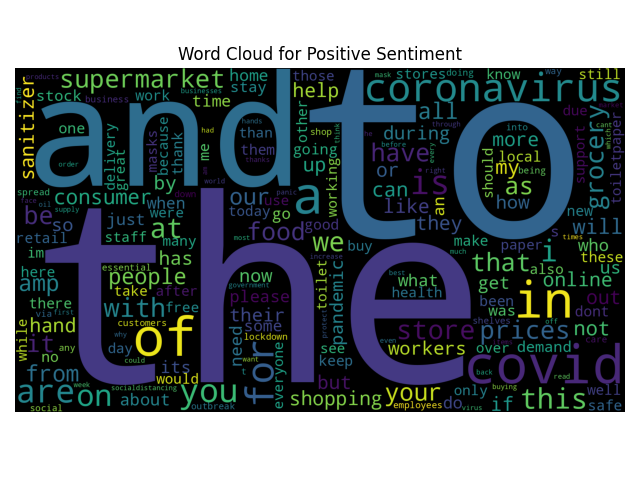
\includegraphics[width=0.8\textwidth]{Assignment 2/q1/wordcloud_Positive.png}
\end{figure}

\begin{figure}[H]
\centering
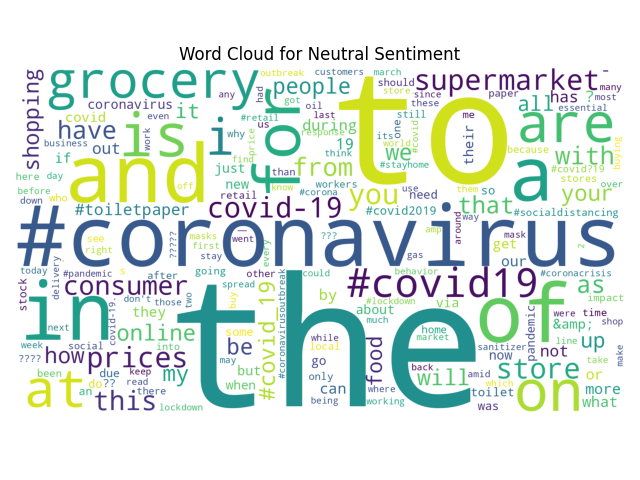
\includegraphics[width=0.8\textwidth]{Assignment 2/q1/wordcloud_Neutral.png}
\end{figure}

\begin{figure}[H]
\centering
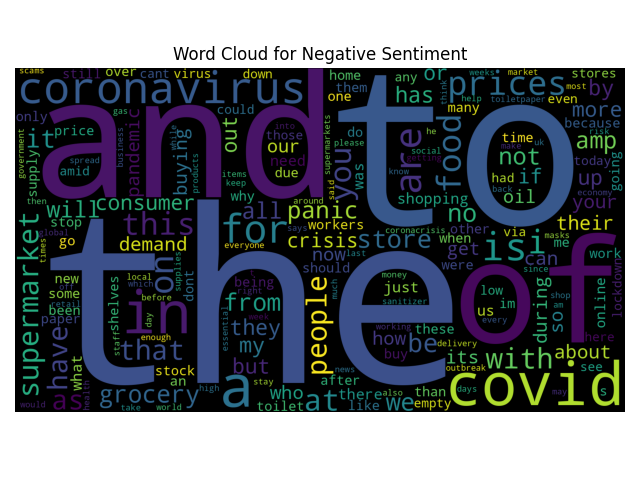
\includegraphics[width=0.8\textwidth]{Assignment 2/q1/wordcloud_Negative.png}
\end{figure}


\subsection{Random and Positive Baseline Accuracy}
\begin{itemize}
    \item Random:
    \begin{itemize}
        \item Training: 33.32 percent
        \item Validation: 32.82 percent
    \end{itemize}

    \item Positive:
    \begin{itemize}
        \item Training: 43.84 percent
        \item Validation: 43.85 percent
    \end{itemize}
\end{itemize}

For three classes, the accuracy of random guessing is:
\begin{equation}
\text{Accuracy} = \frac{1}{3}
\end{equation}

The accuracy when predicting all samples as positive is:
\begin{equation}
\text{Accuracy} = \frac{\text{Number of positive samples}}{\text{Total number of samples}}
\end{equation}

Comparing to the Naive Bayes Classifier I have created, as expected, it performs better than both Random and Positive Prediction.

\begin{table}[h]
    \centering
    \begin{tabular}{|l|c|c|}
    \hline
    \textbf{Method} & \textbf{Training Accuracy} & \textbf{Validation Accuracy} \\
    \hline
    Random & 33.32\% & 32.82\% \\
    \hline
    Positive & 43.84\% & 43.85\% \\
    \hline
    Naïve Bayes & 80.23\% & 69.96\% \\
    \hline
    \end{tabular}
    \caption{Comparison of different methods for text classification.}
    \label{tab:comparison}
\end{table}

The improvement of our Naïve Bayes classifier over:
    \begin{itemize}
        \item Random guessing is \( \approx 34.42\% \).
        \item Predicting all as "Positive" is \( \approx 23.90\% \).
    \end{itemize}



\subsection{Confusion Matrix}

\begin{table}[h]
    \centering
    \begin{tabular}{|c|c|c|c|}
    \hline
     & \textbf{Predicted Positive} & \textbf{Predicted Neutral} & \textbf{Predicted Negative} \\
    \hline
    \textbf{Actual Positive} & True Positives (TP) & False Neutral (FN) & False Negative (FN) \\
    \hline
    \textbf{Actual Neutral} & False Positive (FP) & True Neutrals (TN) & False Neutral (FN) \\
    \hline
    \textbf{Actual Negative} & False Positive (FP) & False Neutral (FN) & True Negatives (TN) \\
    \hline
    \end{tabular}
    \caption{Confusion Matrix Format}
    \label{tab:confusion_matrix}
\end{table}


\subsubsection{Naive Bayes}
\begin{center}
\textbf{Training Set}
\begin{center}
\begin{tabular}{|c|c|c|c|}
\hline
 & Positive & Negative & Neutral \\
\hline
Positive & 14770 & 1565 & 267 \\
\hline
Negative & 1699 & 12252 & 215 \\
\hline
Neutral & 2238 & 1500 & 3358 \\
\hline
\end{tabular}
\end{center}

\textbf{Validation Set}
\begin{center}
\begin{tabular}{|c|c|c|c|}
\hline
 & Positive & Negative & Neutral \\
\hline
Positive & 1196 & 226 & 22 \\
\hline
Negative & 254 & 952 & 26 \\
\hline
Neutral & 290 & 171 & 156 \\
\hline
\end{tabular}
\end{center}
\end{center}

\subsubsection{Random}
\begin{center}
\textbf{Training Set}
\begin{center}
\begin{tabular}{|c|c|c|c|}
\hline
 & Positive & Negative & Neutral \\
\hline
Positive & 5575 & 5528 & 5499 \\
\hline
Negative & 4834 & 4689 & 4643 \\
\hline
Neutral & 2407 & 2337 & 2352 \\
\hline
\end{tabular}
\end{center}

\textbf{Validation Set}
\begin{center}
\begin{tabular}{|c|c|c|c|}
\hline
 & Positive & Negative & Neutral \\
\hline
Positive & 465 & 505 & 474 \\
\hline
Negative & 401 & 427 & 404 \\
\hline
Neutral & 205 & 223 & 189 \\
\hline
\end{tabular}
\end{center}
\end{center}

\subsubsection{Positive}
\begin{center}
\textbf{Training Set}
\begin{center}
\begin{tabular}{|c|c|c|c|}
\hline
 & Positive & Negative & Neutral \\
\hline
Positive & 16602 & 0 & 0 \\
\hline
Negative & 14166 & 0 & 0 \\
\hline
Neutral & 7096 & 0 & 0 \\
\hline
\end{tabular}
\end{center}

\textbf{Validation Set}
\begin{center}
\begin{tabular}{|c|c|c|c|}
\hline
 & Positive & Negative & Neutral \\
\hline
Positive & 1444 & 0 & 0 \\
\hline
Negative & 1232 & 0 & 0 \\
\hline
Neutral & 617 & 0 & 0 \\
\hline
\end{tabular}
\end{center}
\end{center}


\begin{enumerate}
	\item Naive Bayes:

\begin{itemize}
		\item Training Set: The category with the highest value on the diagonal is Positive with 14770 correct predictions.
		\item Validation Set: The category with the highest value on the diagonal is Positive with 1196 correct predictions.
\end{itemize}

	\item Random:

\begin{itemize}
		\item Training Set: The category with the highest value on the diagonal is Positive with 5575 correct predictions.
		\item Validation Set: The category with the highest value on the diagonal is Positive with 465 correct predictions.
\end{itemize}

	\item Positive:

\begin{itemize}
		\item Training Set: The category with the highest value on the diagonal is Positive with 16602 correct predictions.
		\item Validation Set: The category with the highest value on the diagonal is Positive with 1444 correct predictions.
\end{itemize}

\end{enumerate}
The highest value on the diagonal entry indicates that this category was the most accurately predicted among the three. For all three methods (Naive Bayes, Random, and Positive), the "Positive" category has the highest number of correctly predicted instances. This means that the model is best at correctly identifying positive samples.




\subsection{Stopword Removal and Stemming}
\subsubsection{Data Transformation}
Stop Word removal is performed using the set of English stop words in the nltk corpus. Stemming is done using PorterStemmer from nltk.stem.

\subsubsection{Word Clouds}
\begin{figure}[H]
\centering
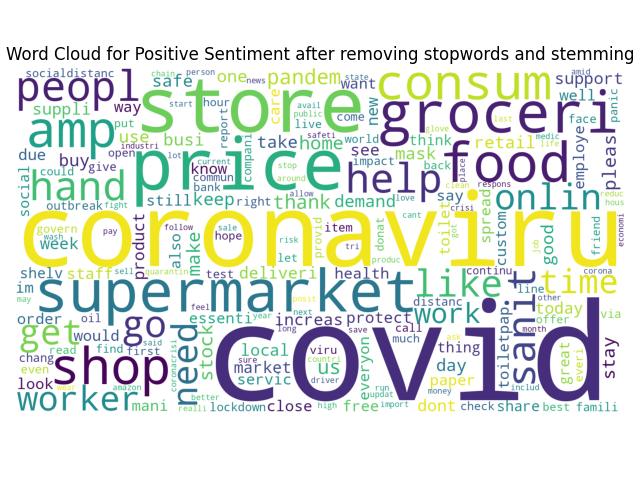
\includegraphics[width=0.8\textwidth]{Assignment 2/q1/wordcloud_Positive_stemming_and_removeStopwords.png}
\end{figure}

\begin{figure}[H]
\centering
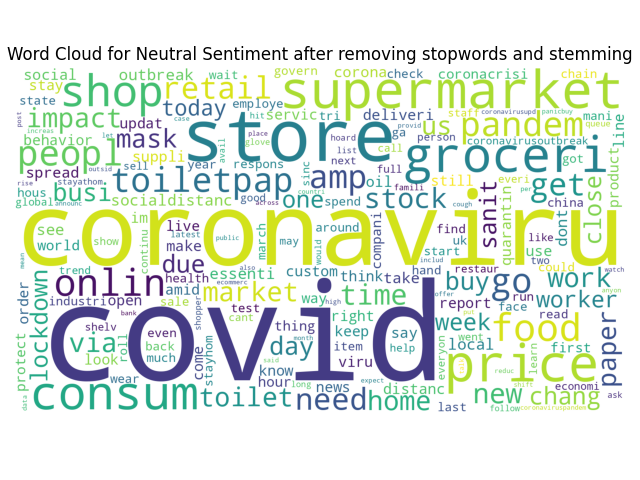
\includegraphics[width=0.8\textwidth]{Assignment 2/q1/wordcloud_Neutral_stemming_and_removeStopwords.png}
\end{figure}

\begin{figure}[H]
\centering
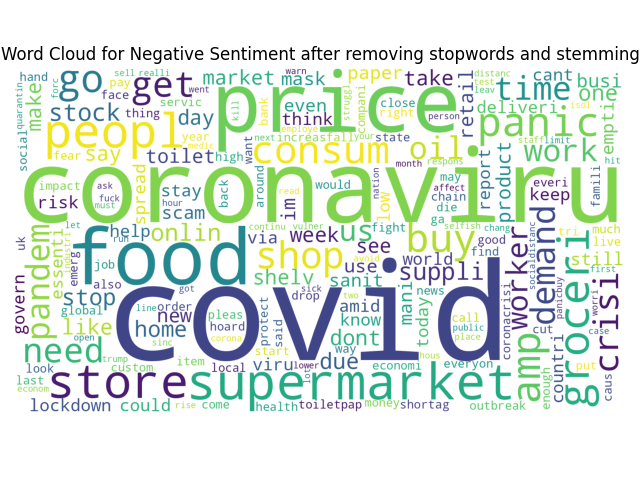
\includegraphics[width=0.8\textwidth]{Assignment 2/q1/wordcloud_Negative_stemming_and_removeStopwords.png}
\end{figure}

\subsubsection{Model Accuracy}
\begin{itemize}
    \item Training: 73.46 percent
    \item Validation: 65.65 percent
\end{itemize}

\subsubsection{Observations}
The wordclouds created after removing stop words and stemming more accurately represent the words with positive and negative sentiment. However, validation accuracy decreases slightly. 

Here are a few potential reasons for this reduction:

\begin{enumerate}
	\item Loss of Contextual Information: By removing stopwords, we may have inadvertently removed some contextual information from the tweets. In some cases, stopwords can provide valuable context. For instance, the phrase "not good" is negative, but if we remove the stopword "not", the sentiment could be misinterpreted.
	\item Over-Stemming: Stemming can sometimes be aggressive, merging words that should be distinct. This can lead to loss of valuable information. For example, the words "universe" and "university" might both be stemmed to "univers", even though they have very different meanings.
	\item Variability in Data: The nature of tweets is such that many words or phrases are used in a colloquial or slang manner. Some of these might be treated as stopwords or might get inappropriately stemmed, leading to loss of sentiment information.
	\item Model Simplicity: The Naïve Bayes classifier assumes that features (words, in this case) are independent given the class label. This is a strong assumption, especially for textual data where word order and context matter. The preprocessing might exacerbate the impact of this assumption by removing or altering words that provide context.
\end{enumerate}


\subsection{Feature Engineering}
% Write your answers for part 1(e) here.

\subsection{Domain Adaptation}
% Write your answers for part 1(f) here.

\section{Image Classification}
\subsection{Binary Classification}
\subsubsection{Using CVXOPT, Linear Kernel}
\text{Given the standard SVM dual formulation:}

\begin{align*}
\max_{\alpha} & \sum_{i=1}^{m} \alpha_i - \frac{1}{2} \sum_{i=1}^{m} \sum_{j=1}^{m} y^{(i)} y^{(j)} \alpha_i \alpha_j \langle x^{(i)}, x^{(j)} \rangle
\end{align*}

\text{subject to:}

\begin{align*}
0 & \leq \alpha_i \leq C, \\
\sum_{i=1}^{m} \alpha_i y^{(i)} & = 0
\end{align*}

\text{The CVXOPT standard quadratic problem format is:}

\begin{align*}
\min_{\alpha} & \frac{1}{2} \alpha^T P \alpha + q^T \alpha
\end{align*}

\text{subject to:}

\begin{align*}
G\alpha & \leq h, \\
A\alpha & = b
\end{align*}

\text{To put the SVM dual in this form:}

\begin{itemize}
\item \( P \) is an \( m \times m \) matrix where \( P_{ij} = y^{(i)} y^{(j)} \langle x^{(i)}, x^{(j)} \rangle \)
\item \( q \) is an \( m \) sized column vector with all elements being -1.
\item \( G \) is a \( 2m \times m \) matrix constructed such that it considers both \( \alpha_i \geq 0 \) and \( \alpha_i \leq C \).
\item \( h \) is a \( 2m \) sized vector with first \( m \) elements being 0 and next \( m \) elements being \( C \).
\item \( A \) is a \( 1 \times m \) row vector with elements as the labels \( y^{(i)} \).
\item \( b \) is a scalar 0.
\end{itemize}


\[ w = \sum_{i=1}^{m} \alpha_i y^{(i)} x^{(i)} \]


For a chosen support vector \( x_s \): \\
\[ b = y_s - \sum_{i=1}^{m} \alpha_i y^{(i)} \langle x^{(i)}, x_s \rangle \]
Ensure \( 0 < \alpha_s < C \) for the chosen \( x_s \).

\[ \text{prediction} = \text{sign}(\langle w, x \rangle + b) \]

\paragraph{Results:}
\begin{itemize}
    \item Number of Support Vectors Obtained: 2383
    \item Percentage of training samples constituting support vectors: 50.06 percent
    \item Intercept (b)= 1.041890005986661
    \item The Validation accuracy came to be 77.5 percent.
    \item 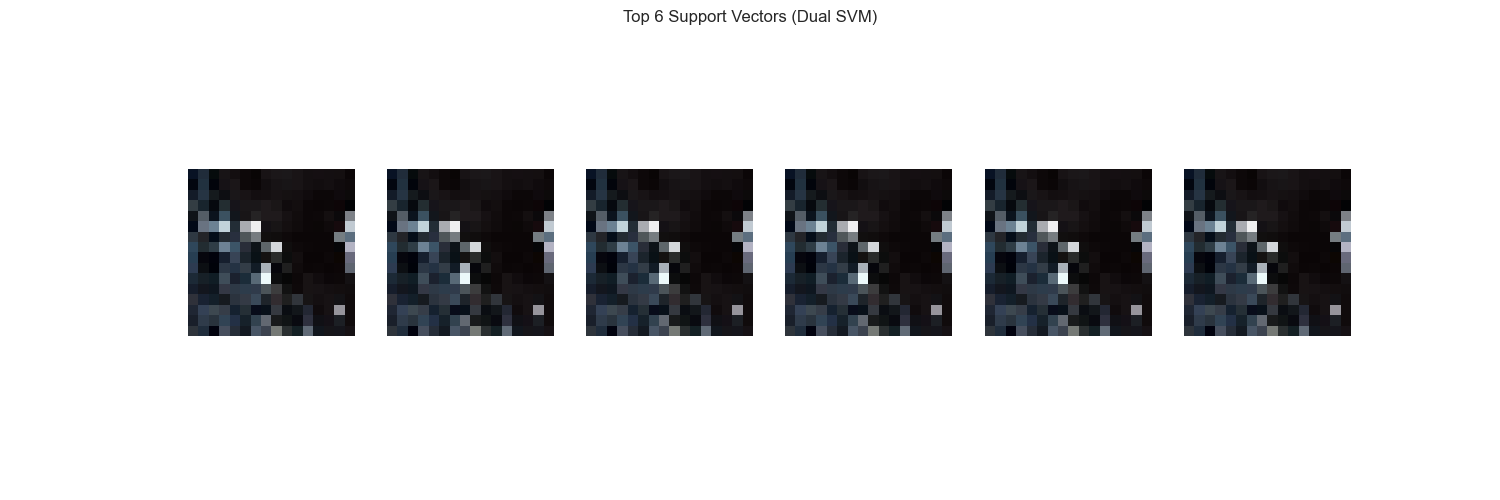
\includegraphics[width=\textwidth]{Assignment 2/q2/top_6_support_vectors_dual cvxopt linear.png}
    \item 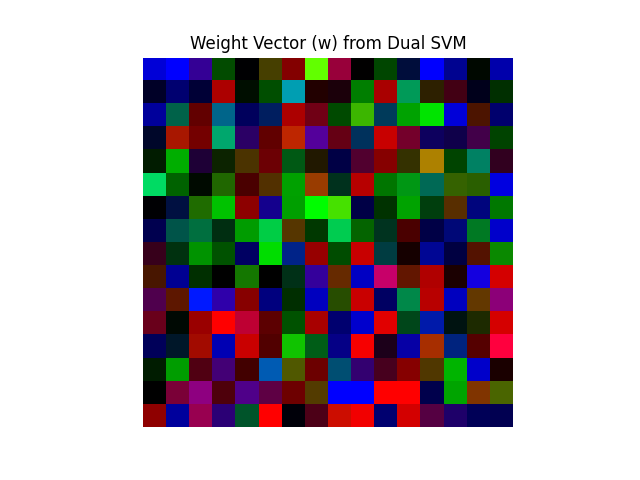
\includegraphics[width=\textwidth]{Assignment 2/q2/weight_vector_dual cvxopt linear.png}
\end{itemize}

\subsubsection{Using CVXOPT, Gaussian Kernel}


\subsubsection{Using scikit-learn SVM function, Linear Kernel}

\paragraph{Results:}
\begin{itemize}
    \item Number of Support Vectors Obtained: 2371
    \item Percentage of training samples constituting support vectors: 49.81 percent
    \item Intercept (b)= 1.06989668
    \item The Validation accuracy came to be 78 percent.
    \item 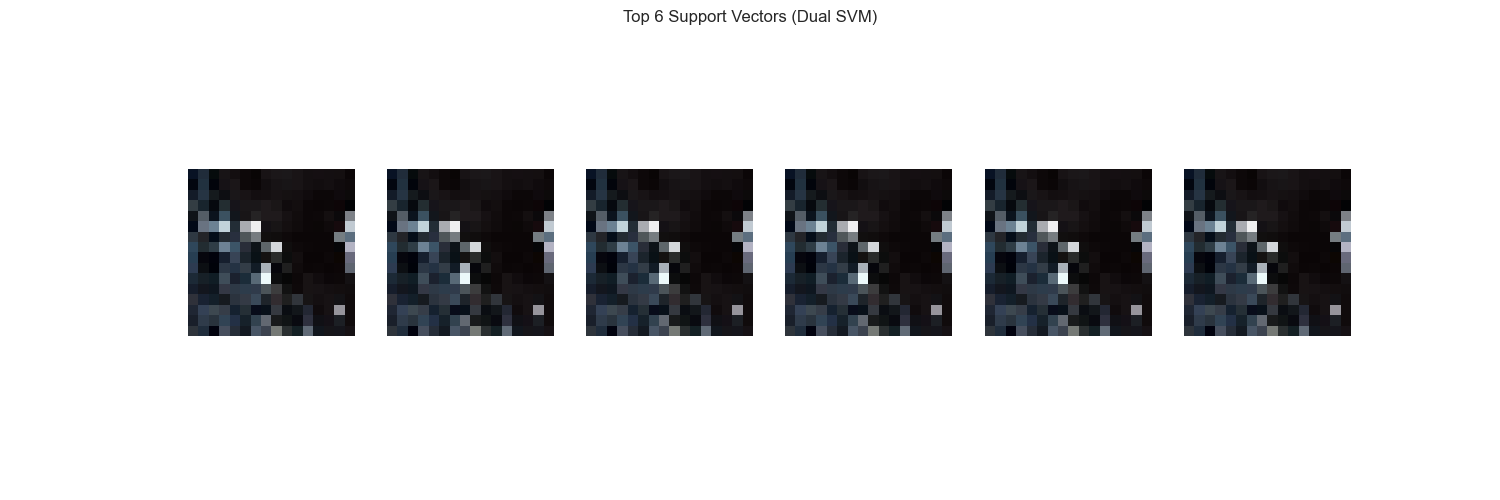
\includegraphics[width=\textwidth]{Assignment 2/q2/top_6_support_vectors_dual cvxopt linear.png}
    \item 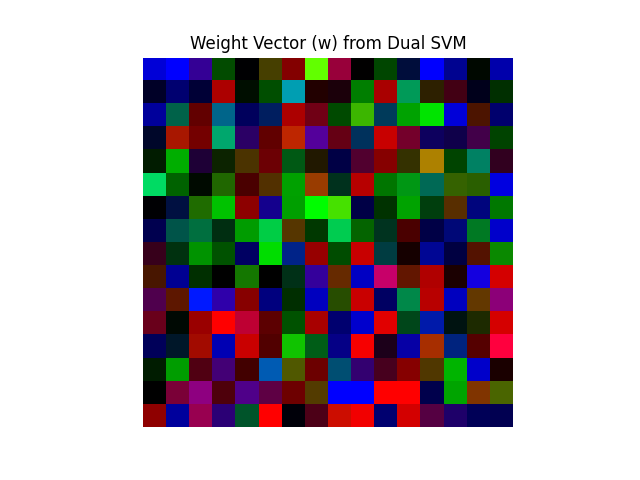
\includegraphics[width=\textwidth]{Assignment 2/q2/weight_vector_dual cvxopt linear.png}
\end{itemize}

\subsubsection{Using scikit-learn SVM function, Gaussian Kernel}

\subsection{Multi-Class Image Classification}
\subsubsection{One-vs-One Multi-Class SVM}
% Write your answer for part 2(a)i here.

\subsubsection{Using scikit-learn SVM function}
% Write your answers for part 2(b) here.

\subsubsection{Confusion Matrix and Observations}
% Write your answers for part 2(c) here.

\subsubsection{Validation and Cross-Validation}
% Write your answers for part 2(d) here.

\section*{Conclusions}
% Summarize your findings and observations here.

\end{document}
